\documentclass[tikz,border=10pt]{standalone}
\begin{document}
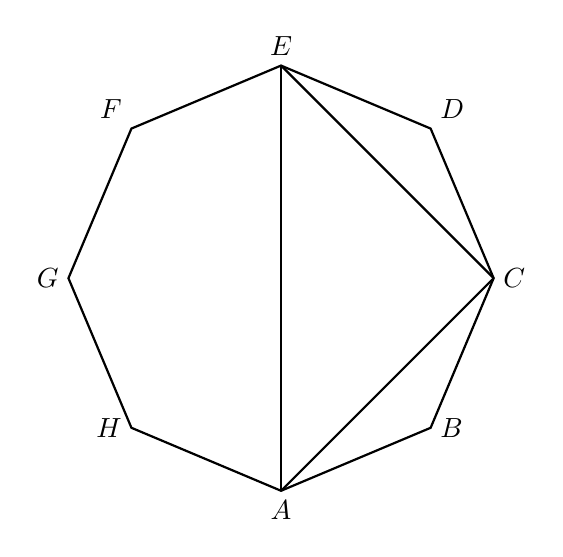
\begin{tikzpicture}[scale=1]
  \coordinate (A) at (4,0);
  \coordinate (B) at (5.9,0.8);
  \coordinate (C) at (6.7,2.7);
  \coordinate (D) at (5.9,4.6);
  \coordinate (E) at (4,5.4);
  \coordinate (F) at (2.1,4.6);
  \coordinate (G) at (1.3,2.7);
  \coordinate (H) at (2.1,0.8);

  \draw[thick] (A) -- (B) -- (C) -- (D) -- (E) -- (F) -- (G) -- (H) -- cycle;
  \draw[thick] (A) -- (E);
  \draw[thick] (A) -- (C);
  \draw[thick] (E) -- (C);

  \node[below] at (A) {$A$};
  \node[right] at (B) {$B$};
  \node[right] at (C) {$C$};
  \node[above right] at (D) {$D$};
  \node[above] at (E) {$E$};
  \node[above left] at (F) {$F$};
  \node[left] at (G) {$G$};
  \node[left] at (H) {$H$};
\end{tikzpicture}
\end{document}
